%%%%%%%%%%%%%%%%%%%%%%%%%%%%%%%%%%%%%%%%%%%%%%%%%%%%%%%%%%%%%%%
%
% Welcome to Overleaf --- just edit your LaTeX on the left,
% and we'll compile it for you on the right. If you open the
% 'Share' menu, you can invite other users to edit at the same
% time. See www.overleaf.com/learn for more info. Enjoy!
%
%%%%%%%%%%%%%%%%%%%%%%%%%%%%%%%%%%%%%%%%%%%%%%%%%%%%%%%%%%%%%%%
\documentclass[12pt, letterpaper]{article}
\usepackage{graphicx} %LaTeX package to import graphics
\graphicspath{{images/}} %configuring the graphicx package
\title{My first LaTeX document}
\author{Hubert Farnsworth\thanks{Funded by the Overleaf team.}}
\date{August 2022}
\begin{document}
    \maketitle
    We have now added a title, author and date to our first \LaTeX{} document!

    Some of the \textbf{greatest}
    discoveries in \underline{science}
    were made by \textbf{\textit{accident}}.

    Some of the greatest \emph{discoveries} in science
    were made by accident.

    \textit{Some of the greatest \emph{discoveries}
    in science were made by accident.}

    \textbf{Some of the greatest \emph{discoveries}
    in science were made by accident.}
    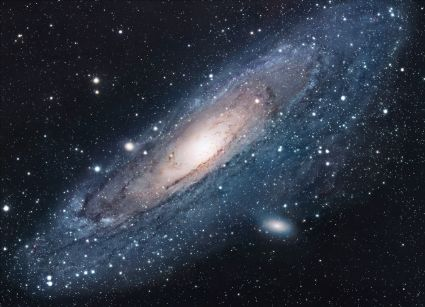
\includegraphics{universe}

    \begin{itemize}
        \item The individual entries are indicated with a black dot, a so-called bullet.
        \item The text in the entries may be of any length.
    \end{itemize}

    \begin{enumerate}
        \item This is the first entry in our list.
        \item The list numbers increase with each entry we add.
    \end{enumerate}

\end{document}